\chapter{Installation of AOM}

We generate shifted beams by sending the seed light through an Acousto-optic Frequency Shifter (AOM)\footnote{haha. Acousto-optic modulator.} using a double pass configuration.\footnote{see figure}. 


It is crucially important that we not put too much intensity through the AOM. 

The AOM we used was a TEF-2500-200-405 made by Brimrose Corporation of America. \footnote{The crystal material was Tellurium Flouride, the center carrier frequency is 2500 MHz, the bandwidth (3dB) was 200 MHz the wavelengtht that it and the associated AR coatings was designed for was 405 nm.} 

\section{Principle of Operation}

The AOM is a crystal with a piezoelectric transducer attached to one side and an acoustic absorber attached to the other side. Acoustic waves are produced by the tranducer. These waves travel across the active area of the AOM crystal and are absorbed by the absorber on the other side. The compression and decompression caused by the travelling acoustic waves changes the index of refraction at various points within the crystal. The resulting alternating pattern of areas of higher and lower index of refraction gives a travelling grating off of which the light can experience Bragg reflection. Because the effective reflective surface is moving, the light scattered off these features is Doppler-shifted and emerges at a distinct angle compared to the incoming light. This allows the AOM to produce frequency-shifted beams. 

The calculation of this is straightforward: 

SHOULD I INCLUDE THE DERIVATION OF THE RELATIONSHIP BETWEEN DRIVING FREQUENCY, ANGLE OF DEFLECTION AND FREQUENCY SHIFT? 

Ultimately, getting the AOM to work properly involves optimizing just a few parameters. We must ensure that the AOM is installed at the right angle relative to the incoming beam. We must ensure that as much of the incoming beam as possible hits the active area of the AOM. This requires alignment in the X and Y dimensions, but it also means that we attempt to maneuver the AOM so that the focal point of the incoming beam is approximately in the center of the crystal. The power used to drive the piezoelectric transducer must be optimized. Furthermore, the intensity and shape of the incoming beam must be adjusted to ensure that we do not exceed the maximum allowable intensity for the AOM, which is specified as 50 W/mm$^2$.
%shape instead of waist?
Thus, we will first discuss some work we did to characterize our incoming beam.

\section{Optimization of Beam Waist}
First, we would like to control our beam so that, at its focus, the majority of the beam fits within the active area of the AOM \footnote{I did explore the possibility of just sending in a huge beam with lots of extra power in hopes that the part scattering off the active part of the AOM would work. Preliminary tests showed little promise for the technique. Furthermore, there is no reason to believe we would get any kind of good mode from this.} This area is spec'd as being .05 mm wide. Thus, we hope for a beam waist radius that will be $\approx$4 times smaller.   

If we take measurements of the beam's waist at several points along the beam's path, we can fit this to the equation given in \cite{SiegmanBeamQuality}. When we do our fit, we can either try to allow $M^2$ to be one of the fit parameters. However, if we constrain $M^2=1$ in our fit, we will end up with a worst-case minimum beam waist radius. 

According to \cite{SiegmanBeamQuality}, the second-moment width, defined as 
\begin{equation}
\sigma_x^2=\frac{\int_{-\infty}^{\infty} (x-x_0)^2 I(x,y)\, dx\, dy}{\int_{-\infty}^{\infty} I(x,y)\, dx \, dy}
\end{equation} 

propagates according to 
\begin{equation}
\sigma_x^2=\sigma_{0x}^2+\left( \frac{M_x^2 \,\lambda}{\pi \, \sigma_{0x}}\right)^2 (z-z_{0x})^2 \label{SiegmanBeamPropagate00}
\end{equation}
 
where $I(x,y)$ is the intensity profile of our beam, which is propagating in the $z$ direction. 

We can look at the effective slope of divergence by rearranging Eq.\ \ref{SiegmanBeamPropagate00} and taking the limit as $(z-z_0) \rightarrow \infty$
\begin{equation}
\frac{\sigma_x}{z-z_0}=M_x^2 \frac{\lambda \pi}{\sigma_{0x}} \label{SiegmanBeamSlope}
\end{equation}
%does z0 matter as a fit parameter? I don't think so. 

From this we see that the minimum possible beam waist radius corresponding to a given beam divergence corresponds to $M^2=1$. Thus, if we assume $M^2=1$, we get a worst-case scenario as far as intensity goes. 

To estimate the intensity, we will first suppose that we have a non-twisted Gaussian beam with waists $w_{x0}=2 \sigma_{x0}$ and $w_{y0}=2 \sigma_{y0}$. The maximum intensity in such a beam in terms of the total power contained in the beam is given by integrating the intensity of the beam. We know that the intensity profile of such a beam has the form\footnote{well, based on Wikipedia and assumptions about Siegman's conventions}:

\begin{equation}
I(x,y)=({\rm constants}) \exp \left( -2 \left(\frac{x}{W_{0x}} \right)^2-2 \left( \frac{y}{W_{0y}}\right)^2\right). \label{intensityEquation}
\end{equation}

We can find the value of the constants by integrating\footnote{maybe I shouldn't have this in here, it's too simple. I always have to double check my coefficients and factors of 2, though, so the equations should definitely at least be there}: 

\begin{align}
{\rm Total\ Power}=P&=\int_{-\infty}^\infty I(x,y)\, dx\, dy\\
&=\frac{\pi}{2}({\rm constants}) W_{0x} W_{0y}
\end{align}

We can solve for our constants and rewrite them in terms of $P$, $W_{0x}$ and $W_{0y}$ we find that Eq.\ \ref{intensityEquation} becomes 

\begin{equation}
I(x,y)= \frac{2 P}{\pi W_{0x} W_{0y}}\exp \left( -2 \left(\frac{x}{W_{0x}} \right)^2-2 \left( \frac{y}{W_{0y}}\right)^2\right). \label{intensityEquation2}
\end{equation}

We thus see that the maximum intensity of such a beam is $2P/\pi W_{0x}W_{0y}$.

We can measure the beam-waist radius using a standard knife-edge technique. By integrating, we see that the appropriate function to fit to is 

\begin{equation}
{\rm Power\ incident\ on\ photodiode}=\frac{1}{2} P \left(\erf \left( \frac{\sqrt{2} x}{W_{0x}}\right)\right)
\end{equation}


The values thusly obtained can then be fitted to Eq.\ \ref{SiegmanBeamPropagate00}. This is done in an appendix. 


The possibility of using a camera exists. There is an appendix with information about my failed attempt to calibrate a non-scientific camera. 


\subsection{Ray Transfer Matrix Analysis of System}
As a sanity check, we can calculate using an ABCD matrix (ray-transfer matrix) what the beam waist should be for our optical setup. This model can be used to estimate our sensitivity to small changes in the setup. 

%This is in a lab notebook somewhere. You need to find it there, I think. Or it's in a Mathematica file. 
%found: the Mathematica files are generalABCDfinding.nb, ABCDwillWeBreakAOM.nb . The m files, well, I think the ones I want are in checkTheWaists_realDATA. 

According to \cite{SiegmanBeamQuality}, we can model the propagation of the ``embedded'' Gaussian beam. We could then, in principle, model our beam based on our knowledge of the $M^2$. However, recall that in our analysis, we've been assuming a sort of worst case scenario $M^2=1$. Thus, we will model our beam call the well-known rule for modelling the change of a Gaussian beam as it passes through a system described by ray transfer matrix with coefficients $A$,$B$,$C$ and $D$, which is 

\begin{equation}
z'-iz_0'=\frac{A(z-iz_0)+B}{C(z-iz_0)+D}
\end{equation}
\cite{BYUOpticsBook}

which can be solved to give 

\begin{align}
z_0' &= \frac{ z_0 (BC-AD)}{C^2z^2+C^2z_0^2+2 C D z + D^2} \\
z' &=\frac{AC z^2+ACz_0^2+ADz+BCz+BD}{C^2z^2+C^2z_0^2+2 C D z + D^2}
\end{align}

This calculation should give us a feel for how sensitive we are to drifts in the optical setup. We will also be able to compare the results of this calculation to the measured values. 

The system has only a few components that we need to model. At the start, we assume that the light coming out of the face of the laser diode is essentially a Gaussian beam with different beam waist radii for the $x$ and $y$ directions. We see in the datasheet (of the SHARP laser, which isn't even the laser that's in there, necessarily) that the laser's angle of divergence coming out of the lens (LOOK THIS UP) is going to be XXX and XXX. A Gaussian beam's angular divergence can be surmised by looking at Eq.\ \ref{SiegmanBeamSlope}. The relationship turns out to be \cite{MellesGriotGaussian}. Well, a few issues: I'm not sure if the Gaussian beam crap holds at this angle because it's sort of a large angle of divergence. Also, wait, no it's not that large of an angle of divergence. Well, the point is, one can use the given angle of divergence of light from the laser diode in order to infer what the equivalent Gaussian beam radii are. These turn out to be 972.913 nm and 460.854 nm. 

The light from the laser head is emitted and collimated by a lens\footnote{Thorlabs C570TM-A} with focal point 2.84 mm.%before, I had 2.87 mm, IDK why
 The beam goes through various components whose collective impact can be modeled as mere propagation 
\footnote{Even though propagating through a medium like the crystals in our isolators is different than propagating through air, travelling some distance through any medium is the same as travelling some effective distance through air. Since we can't measure the total path length very accurately anyway, we just fold the propagation through these crystals into the overall propagation}
through some effective distance that should be on the order of 1 m. The beam is then focused by a lens with focal length 10 cm and passed through the AOM. 

We can write the ABCD matrix for the whole system as the following product of ABCD matrices: 

\begin{equation}
\begin{bmatrix}
1 & 0 \\ -1/f_{f} & 1
\end{bmatrix}
\begin{bmatrix}
1 & d_2-d_1 \\ 0 & 1
\end{bmatrix}
\begin{bmatrix}
1 & 0 \\ -1/f_{a} & 1
\end{bmatrix}
\begin{bmatrix}
1 & d_1 \\ 0 & 1
\end{bmatrix}
=
\begin{bmatrix}
A & B \\ C & D
\end{bmatrix}
\end{equation}

Of course, finding the actual result is straightforward, though writing it out would be unenlightening because it is algebraically messy. Thus, we used Mathematica to find the expressions for $z_0'$ and $z'$ and then copied and pasted these expressions into an Octave function. This can then be evaluated for realistic values of $d_1$ (the distance from the laser face to the collimating lens) and $d_2$ (the distance traveled between the collimating lens and the other lens). 

From this analysis, we calculate the effective area of our beam and the corresponding ratio between the intensity at the most intense part of the beam and the total power in the beam. If we see that these ratios do not change too much for reasonable parameters, we need not fear that a slight change in the position of one of our optical elements will be disastrous:


\begin{figure}
    %\centerline{\includegraphics[trim=100pt 100pt 100pt 100pt, clip=true, totalheight=0.5\textheight,angle=90]{testfigure}}
    %\centerline{\includegraphics[totalheight=0.3\textheight]{testfigure}}
    \centerline{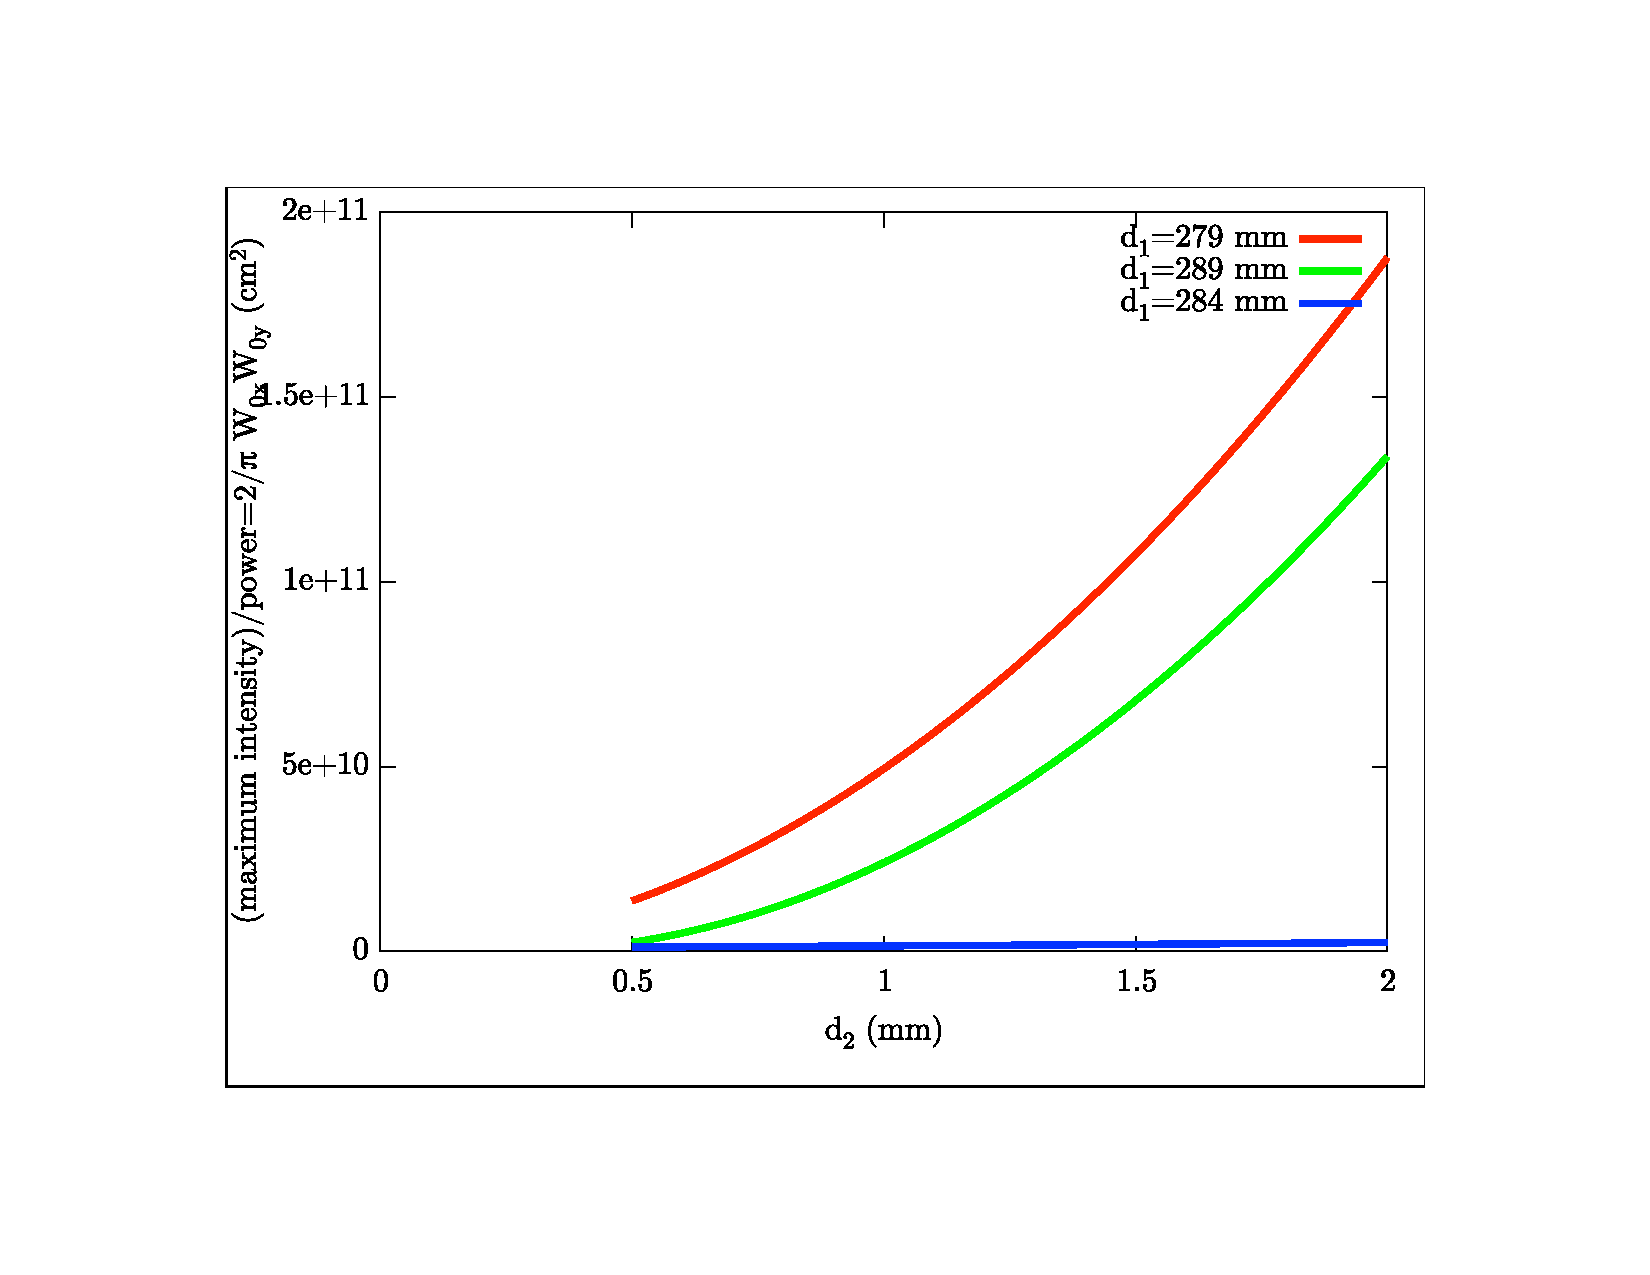
\includegraphics{waists1}}
    %\includegraphics[totalheight=0.3\textheight]{testfigure}
    \caption[]{\label{fig:typicaldata}
    TBA}
\end{figure}

\begin{figure}
    %\centerline{\includegraphics[trim=100pt 100pt 100pt 100pt, clip=true, totalheight=0.5\textheight,angle=90]{testfigure}}
    %\centerline{\includegraphics[totalheight=0.3\textheight]{testfigure}}
    \centerline{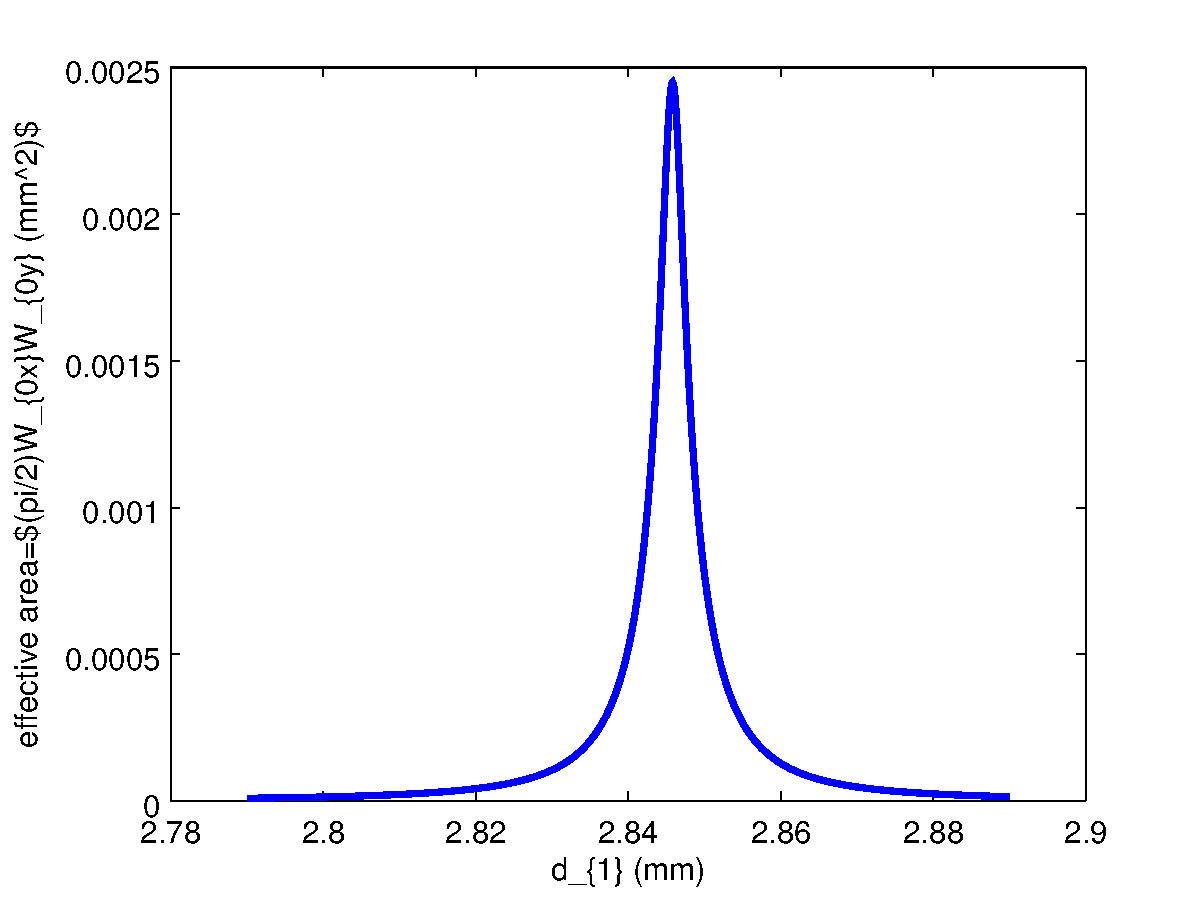
\includegraphics{waists2}}
    %\includegraphics[totalheight=0.3\textheight]{testfigure}
    \caption[]{\label{fig:typicaldata}
    TBD}
\end{figure}




We can talk about that camera. That could be good. %everything is easy once you do it.
